\documentclass[11pt]{article}
\usepackage[utf8]{inputenc}
\usepackage[T1]{fontenc}
\usepackage{graphicx}
\usepackage{float}
\usepackage{booktabs} % For better looking tables
\usepackage{graphicx}
\usepackage[table]{xcolor}
\usepackage{array}
\title{Sécurité Alimentaire B : Comprendre les Nutriments Essentiels et Leur Importance}

\begin{document}

\maketitle

\section{Nutriments Essentiels}
Tous les nutriments sont vitaux pour le fonctionnement optimal du corps. Cependant, certains nutriments sont classifiés comme "essentiels" parce que le corps ne peut pas les synthétiser en quantités adéquates.\\
Ceux-ci incluent :

\begin{itemize}
    \item[-] Vitamines : Les formes solubles dans l'eau et dans les graisses.
    \item[-] Minéraux alimentaires et oligo-éléments.
    \item[-] Certains acides aminés : Isoleucine, leucine, lysine, méthionine, phénylalanine, thréonine, tryptophane, valine, et histidine.
    \item[-] Certains acides gras : Acide linoléique (oméga-6) et acide alpha-linolénique (oméga-3).
\end{itemize}

\section{Besoins en Nutriments}
Les besoins en nutriments varient selon l'âge, le genre, le niveau d'activité physique, les habitudes alimentaires, le statut physiologique (par exemple, la grossesse) et la génétique. Par exemple, les végétariens peuvent nécessiter des ajustements dans leur apport en fer par rapport aux mangeurs de viande.

\newpage

\section{Valeurs Nutritionnelles de Référence}
Les valeurs nutritionnelles de référence sont établies sur la base de publications scientifiques. Les experts analysent la relation entre l'apport en nutriments, le statut en nutriments dans le corps, et la santé pour :

\begin{itemize}
    \item[-] Prévenir les carences en nutriments.
    \item[-] Soutenir les fonctions physiologiques et biochimiques.
    \item[-] Offrir une protection contre les maladies non transmissibles (par exemple, les maladies cardiovasculaires).
\end{itemize}

\subsection{Valeurs d'Extrapolation Épidémiologique}
Ces valeurs permettent l'approximation des besoins en nutriments et sont essentielles dans l'adaptation des directives alimentaires.

\section{État Nutritionnel}
L'état nutritionnel reflète l'état physiologique d'un individu, déterminé par l'apport en nutriments, les besoins en nutriments, et la capacité du corps à digérer, absorber, et utiliser les nutriments.

\section{Facteurs Influant sur l'État Nutritionnel}
Divers facteurs peuvent affecter l'état nutritionnel, y compris les maladies chroniques, les troubles alimentaires, les conditions socio-économiques, et l'accès à une nourriture saine. Il est crucial de considérer ces facteurs lors de l'évaluation de l'état nutritionnel.

\section{Stratégies d'Amélioration de la Nutrition}
Améliorer la nutrition nécessite une approche globale, incluant l'éducation nutritionnelle, l'amélioration de l'accès à des aliments sains, et la mise en œuvre de politiques publiques soutenant une alimentation équilibrée.
\section{Résumé sur les protéines}

Les protéines, essentielles pour la construction et la réparation des tissus, diffèrent en qualité nutritionnelle. Cette qualité est jugée sur la digestibilité et la composition en acides aminés essentiels. Les protéines animales sont généralement plus digestibles et complètes en acides aminés par rapport aux protéines végétales. Cependant, en combinant divers aliments végétaux, il est possible d'obtenir un profil complet d'acides aminés. Il est crucial de considérer à la fois la quantité et la qualité des protéines pour une alimentation équilibrée.

\section{Evaluer la qualité des protéines avec le DIAAS (Digestible Indispensable Amino Acid Score)}
\textit{Les pourcentages supérieurs à 100 signifient une quantité excédentaire d'acides aminés essentiels par rapport aux besoins.}
\begin{table}[h!]
    \centering
    \begin{tabular}{@{}llll@{}}
    \toprule
    \textbf{Food Item}        & \textbf{DIAAS (\%)} & \textbf{Quality of Protein} & \textbf{Reference}    \\ \midrule
    Whole Milk Powder         & 143                 & High                        & FAO (2013)            \\
    Milk protein concentrate  & 118                 & High                        & FAO (2013)            \\
    Whole Milk                & 114                 & High                        & Philips (2017)        \\
    Egg – hard boiled         & 113                 & High                        & Philips (2017)        \\
    Beef                      & 111                 & High                        & Ertl et al (2017)     \\
    Whey protein isolate      & 109                 & High                        & FAO (2013)            \\
    Chicken breast            & 108                 & High                        & Philips (2017)        \\
    Soy protein concentrate   & 98.5                & Good                        & Philips (2017)        \\
    Whey protein concentrate  & 98.3                & Good                        & Philips (2017)        \\
    Pea protein               & 91.5                & Good                        & Philips (2017)        \\
    Soy protein               & 91.5                & Good                        & Philips (2017)        \\
    Wheat                     & 91.5                & Good                        & Philips (2017)        \\
    Soy protein isolate       & 90                  & Good                        & Philips (2017)        \\
    Chickpeas                 & 83                  & Good                        & Philips (2017)        \\
    Pea protein concentrate   & 82                  & Good                        & Philips (2017)        \\ \bottomrule
    \end{tabular}
    \caption{Protein Quality Comparison}
    \label{tab:protein_quality}
\end{table}
    
\section{Quelques chiffres}

\subsection{France, étude NutriNet-Santé (2009)}
\begin{itemize}
    \item[-] 15\% des hommes et 28\% des femmes prenaient des compléments alimentaires au moins trois jours par semaine.
    \item[-] 60\% des compléments sont consommés régulièrement depuis plus d'un an.
    \item[-] Dans 55\% des cas, les produits sont conseillés ou prescrits par un médecin.
\end{itemize}

\subsection{Suisse, étude sur la cohorte CoLaus (environ 6000 sujets)}
\begin{itemize}
    \item[-] 26\% des sujets consomment un supplément (vitamines / sels minéraux : 16,8\%).
    \item[-] Les femmes consomment plus de suppléments que les hommes.
    \item[-] La consommation est associée à un meilleur profil de santé.
\end{itemize}

Référence : P Marques-Vidal et al., \textit{European Journal of Clinical Nutrition} (2009) 63.

\section{Efficacité et Objectifs des Suppléments Nutritionnels}

Malgré leur popularité, il existe une « carence » notable d'études scientifiques de haute qualité, telles que les essais cliniques randomisés et les essais en double aveugle, démontrant l'efficacité clinique des suppléments nutritionnels. L'utilisation de ces produits peut être divisée en deux catégories principales :

\subsection{Prescriptions médicales}
Les prescriptions de suppléments par les professionnels de santé s'appuient sur un diagnostic précis et des besoins nutritionnels clairement identifiés. Ces prescriptions ont pour but de gérer les carences nutritionnelles, les insuffisances spécifiques, ou de prévenir la toxicité due à un excès de certains nutriments. Cette approche est fondamentalement basée sur des preuves scientifiques et cliniques solides.

\subsection{Automédication}
L'automédication avec des suppléments est souvent motivée par le désir d'améliorer le bien-être général, la performance physique ou cognitive, de prévenir les maladies, ou de gérer les conséquences de certaines conditions de santé. Cependant, cette pratique manque fréquemment de fondement scientifique et peut être guidée par des informations erronées ou incomplètes.

En résumé, alors que les suppléments nutritionnels peuvent jouer un rôle dans la gestion de certaines conditions de santé et dans la prévention des carences, leur utilisation doit être judicieuse et basée sur des preuves scientifiques pour garantir leur efficacité et leur sécurité.

\section{La Vitamine C et la Lutte contre le Rhume}

Une méta-analyse regroupant 29 études cliniques, impliquant environ 11'300 participants et majoritairement des essais randomisés en double aveugle, a examiné l'effet de la consommation de plus de 0,2 g/jour de vitamine C sur l'incidence et la durée du rhume.

\subsection{Résultats}
Les résultats montrent une réduction modeste de la durée du rhume : 8\% chez les adultes et 14\% chez les enfants. Une consommation de 1 à 2 g de vitamine C par jour a permis une réduction de 18\% de la durée du rhume chez les enfants, ainsi qu'une diminution de la sévérité des symptômes. Cependant, l'effet thérapeutique de la vitamine C sur la durée ou la sévérité du rhume chez les adultes n'a pas été constamment observé.

\subsection{Conclusions}
La supplémentation en vitamine C ne semble pas réduire l'incidence du rhume dans la population générale, rendant une supplémentation systématique non justifiée. Néanmoins, elle pourrait être bénéfique pour les individus subissant de courts épisodes d'effort physique intense. Compte tenu de son faible coût et de sa sécurité, les patients atteints de rhume pourraient tester de manière individuelle l'efficacité thérapeutique de la vitamine C. Des études supplémentaires, notamment des essais randomisés, sont nécessaires pour confirmer ces observations.

\textit{Source: Hemilä H, Chalker E. Vitamin C for preventing and treating the common cold. Cochrane Database of Systematic Reviews 2013, Issue 1. Art.}

\section{Considérations sur les Compléments Alimentaires}

Les compléments alimentaires, reconnus pour être des substances biologiquement actives, soulèvent plusieurs considérations importantes liées à leur utilisation et leur impact sur la santé.

\begin{itemize}
    \item[-] \textbf{Manque d'évidence scientifique :} Il existe un déficit d'études robustes prouvant l'efficacité des compléments alimentaires sur la santé. Cette lacune souligne la nécessité d'une approche prudente lors de leur utilisation.
    
    \item[-] \textbf{Évaluation des besoins nutritionnels :} Avant de recourir à des compléments, il est crucial d'évaluer les besoins nutritionnels réels avec l'aide d'un professionnel de santé. Cette démarche aide à éviter l'automédication, qui peut être risquée.
    
    \item[-] \textbf{Privilégier une alimentation équilibrée :} Une alimentation diversifiée et un mode de vie sain sont fondamentaux. Ils devraient être privilégiés pour répondre aux besoins nutritionnels avant de considérer l'usage de compléments alimentaires.
    
    \item[-] \textbf{Usage ciblé des compléments :} Lorsqu'il est établi qu'un besoin nutritionnel spécifique existe et ne peut être comblé par l'alimentation seule, l'utilisation de compléments peut être envisagée. Cependant, cela doit se faire sous recommandation d'un professionnel de santé qualifié, en prenant en compte la posologie adéquate, ainsi que les interactions potentielles avec le style de vie, les médicaments existants et d'autres micronutriments.
\end{itemize}

En somme, bien que les compléments alimentaires puissent jouer un rôle dans la gestion de besoins nutritionnels spécifiques, leur utilisation doit être judicieuse, basée sur des conseils professionnels et intégrée dans le cadre d'une approche globale de la santé.

\section{Assurer des Apports Nutritionnels par une Alimentation Variée et Équilibrée}

L'importance d'une alimentation variée et équilibrée pour répondre aux besoins nutritionnels est primordiale. Un exemple notable est l'apport en vitamine D, essentiel pour la santé osseuse, l'immunité et d'autres fonctions corporelles. Les ressources alimentaires locales peuvent jouer un rôle clé dans l'apport de cette vitamine.

\subsection{Le cas de la Vitamine D : Exemples de Ressources Locales}

\textbf{Truite de la Gruyère :}
La truite, en particulier celle issue de l'élevage, représente une excellente source de vitamine D. Un filet de 100g de truite peut fournir entre 6.1 et 11.7 mg de vitamine D, couvrant ainsi près de 30 à 50\% des apports recommandés pour un adulte de plus de 60 ans. Cette contribution significative illustre comment des choix alimentaires ciblés peuvent contribuer à l'atteinte des besoins nutritionnels sans recourir systématiquement à des suppléments.

Cet exemple souligne l'importance d'intégrer des aliments variés et nutritifs dans le régime alimentaire pour assurer un apport adéquat en nutriments essentiels, comme la vitamine D, et favoriser ainsi une bonne santé globale.

\begin{table}[h!]
    \centering
    \begin{tabular}{|c|c|c|c|}
    \hline
    Œuf entier Suisse & 25(OH)D\textsubscript{3} $\mu g/100g$ & Vit. D\textsubscript{3} $\mu g/100g$ & Vit. D\textsubscript{3} totale $\mu g/100g$ \\
    \hline
    A & 0.88 & 1.76 & 2.64 \\
    B & 0.84 & 5.78 & 6.62 \\
    C & 1.13 & 6.26 & 7.39 \\
    D & 0.73 & 2.60 & 3.33 \\
    E & 0.82 & 1.31 & 2.13 \\
    F & 1.15 & 4.11 & 5.26 \\
    G & 0.84 & 8.73 & 9.57 \\
    \hline
    \end{tabular}
    \caption{Concentration of Vitamin D dans from Switzerland.}
    \label{table:vitd_eggs}
    \end{table}

\newpage
\section{Le vieillisement de la popuplation: un enjeu majeur pour les polituqes et systèmes de santé}
\begin{figure}[h!]
    \centering
    \begin{minipage}[b]{0.5\textwidth}
      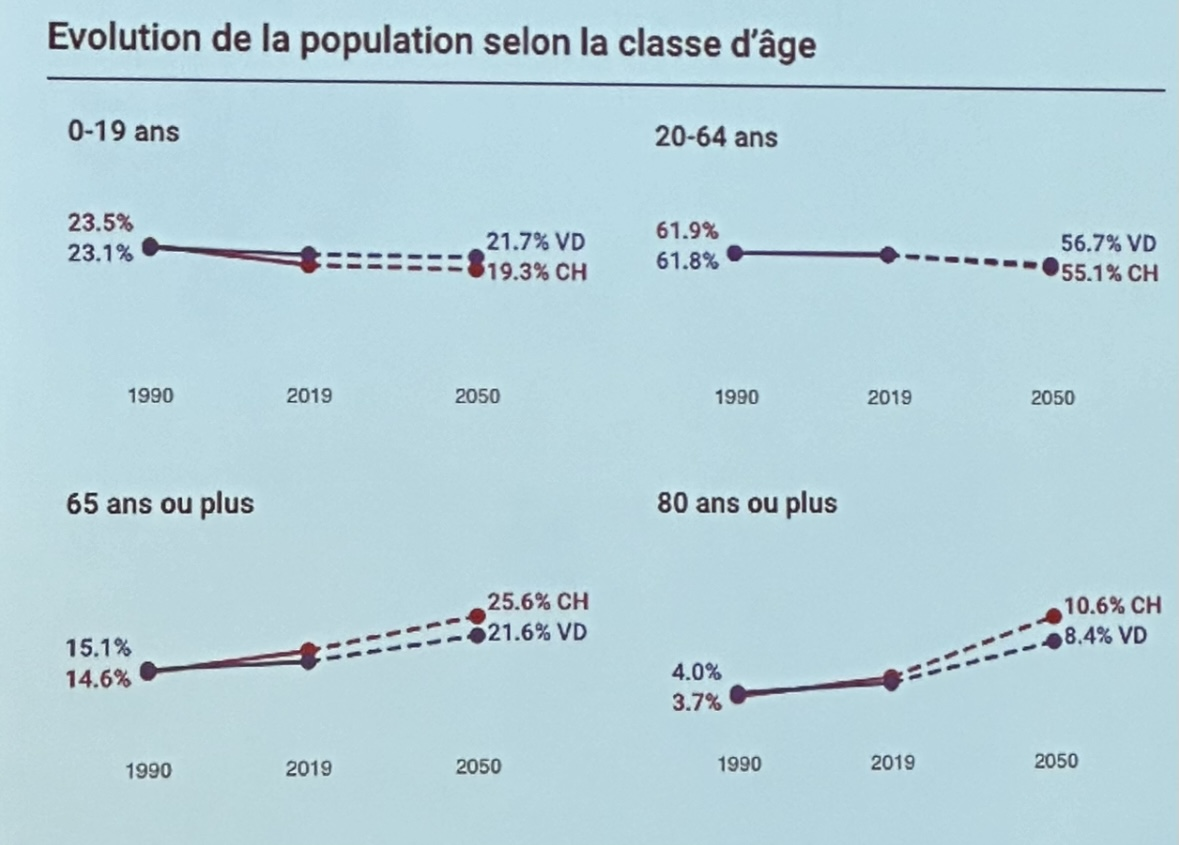
\includegraphics[width=\textwidth]{images/14.jpg}
      \caption{Hassoul première image }
      \label{fig:image1}
    \end{minipage}
    \hfill

    \vspace*{10px}
    \begin{minipage}[b]{0.45\textwidth}
      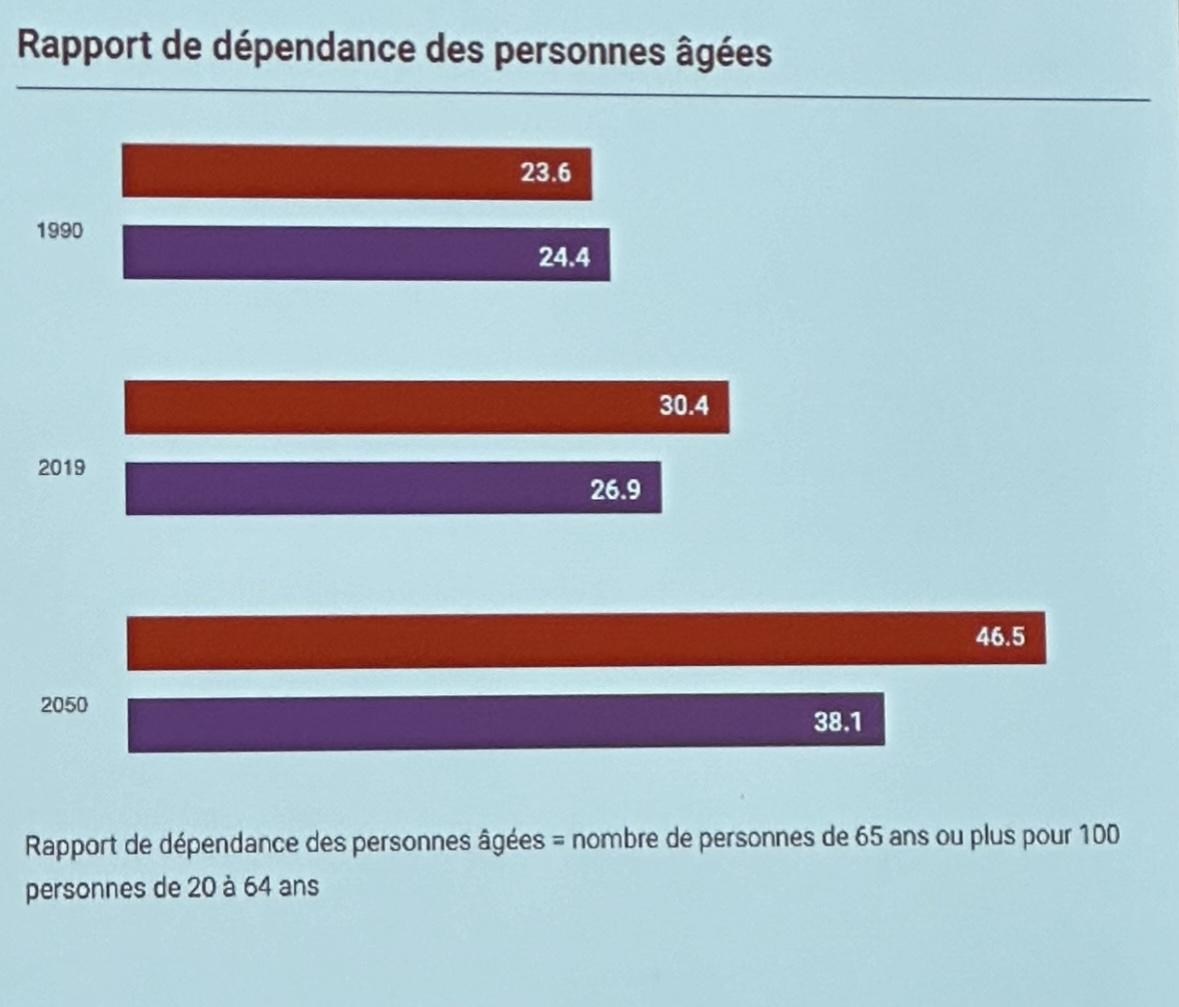
\includegraphics[width=\textwidth]{images/14_2.jpg}
      \caption{hop voilà la deuxieme (un peu flemme d'essayer de capter il a rien écris il a juste parler)}
      \label{fig:image2}
    \end{minipage}
  \end{figure}


  \newpage
  \section{Les mesures de l'obésité}

L'IMC, une mesure simple et répandue au niveau des populations...

L'indice de masse corporelle (IMC) = poids en kg divisé par le carré de la taille en mètres (kg/m$^2$)

\begin{table}[h!]
\centering
\begin{tabular}{|m{3cm}|m{3cm}|m{3cm}|m{3cm}|}
\hline
\rowcolor{green!50}
Normal & Surpoids & Obésité & Obésité morbide \\
\rowcolor{green!25}
18.5-24.9 & 25-29.9 & 30-39.9 & > 40 \\
\hline
\end{tabular}
\caption{Indice de masse corporelle}
\end{table}

\textit{Mais l'IMC est une mesure imparfaite au niveau des individus}

\section{Les conséquences de l'obésité}
Un risque de morbidité accru ammène :
\begin{itemize}
    \item[-] Heart Disease
    \item[-] Lipid Problems
    \item[-] Hypertension
    \item[-] Type 2 diabetes
    \item[-] Dementia
    \item[-] Cancer
    \item[-] Polystic Ovarian Syndrom
    \item[-] Non-Alcoholic Fatty Liver Disease 
\end{itemize}

\section{Les enjeux de prévention de l'obéité, des mesures de lutte à différents niveaux}

\subsection{Au niveau individuel}
\begin{itemize}
    \item[-] limiter l'apport énergétique provenant de la consommation des lipides totaux et de sucres;
    \item[-] consommer d'avantage de fruits et légumes, de légumineuses, de céréales complètes et de noix;
    \item[-] avoir une activité physique régulière (60 minutes par jour pour les enfants et 150 minutes par semaine pour les adultes).
\end{itemize}
\subsection{Au niveau de l'industrie agro-alimentaire}
\begin{itemize}
    \item[-] en réduisant la teneur en sucre, en sel et en graisses saturées des aliments transformés.
    \item[-] en proposant à tous les consommateurs des aliments sains et nutritifs à prix abordables.
    \item[-] en limitant la commercialisation d'aliments riches en lipides, en sel et en sucre, notamment ceux qui sont destinés aux enfant et aux adolescents.
    \item[-] en veillant à proposer des aliments sains et nutritifs et à favoriser une activité physique sur le lieu du travail.
\end{itemize}

\section{Améliorer notre alimentation}
\begin{itemize}
    \item[] Promouvoir une alimentation équilibré et un style de vie saint (activité physique)
    \item[] Reformulation des produits alimentaires afin de réduire les apports en:
    \begin{itemize}
        \item[-] Sel
        \item[-] Sucre
        \item[-] Acides gras
\end{itemize}
    \item[+] Développement et la mise à disposition d'outils simples pour l'optimisation du profil nutritionnel d'un régime alimentaire garantissant:
    \item[+] Apport caloriques ajustés en fonction du genre et du style de vie (activité physique)
    \item[+] Apport suffisants de micronutriments (vitamines, minéraux)
    \item[+] Intégration de l'empreinte écologique

    \end{itemize}   
\end{document}
